\documentclass{article}

  % packages
    % basic stuff for rendering math
    \usepackage[letterpaper, top=1in, bottom=1in, left=1in, right=1in]{geometry}
    \usepackage[utf8]{inputenc}
    \usepackage[english]{babel}
    \usepackage{amsmath} 
    \usepackage{amssymb}
    \usepackage{bookmark}

    % extra math symbols and utilities
    \usepackage{mathtools}        % for extra stuff like \coloneqq
    \usepackage{mathrsfs}         % for extra stuff like \mathsrc{}
    \usepackage{centernot}        % for the centernot arrow 
    \usepackage{bm}               % for better boldsymbol/mathbf 
    \usepackage{enumitem}         % better control over enumerate, itemize
    \usepackage{hyperref}         % for hypertext linking
    \usepackage{xr-hyper}
    \usepackage{fancyvrb}          % for better verbatim environments
    \usepackage{newverbs}         % for texttt{}
    \usepackage{xcolor}           % for colored text 
    \usepackage{listings}         % to include code
    \usepackage{lstautogobble}    % helper package for code
    \usepackage{parcolumns}       % for side by side columns for two column code
    \usepackage{algorithm}
    \usepackage{algpseudocode}
    \usepackage{bbm}
    \algblock{Class}{EndClass}

    % page layout
    \usepackage{fancyhdr}         % for headers and footers 
    \usepackage{uniquecounter}
    \usepackage{lastpage}         % to include last page number in footer 
    \usepackage{parskip}          % for no indentation and space between paragraphs   
    \usepackage[T1]{fontenc}      % to include \textbackslash
    \usepackage{footnote}
    \usepackage{etoolbox}

    % for custom environments
    \usepackage{tcolorbox}        % for better colored boxes in custom environments
    \tcbuselibrary{breakable}     % to allow tcolorboxes to break across pages

    % figures
    \usepackage{pgfplots}
    \pgfplotsset{compat=1.18}
    \usepackage{float}            % for [H] figure placement
    \usepackage{tikz}
    \usepackage{tikz-cd}
    \usepackage{circuitikz}
    \usetikzlibrary{arrows, arrows.meta}
    \usetikzlibrary{positioning}
    \usetikzlibrary{calc}
    \usepackage{graphicx}
    \usepackage{caption} 
    \usepackage{subcaption}
    \captionsetup{font=small} 

    % for tabular stuff 
    \usepackage{dcolumn}

    \usepackage[nottoc]{tocbibind}
    \pdfsuppresswarningpagegroup=1
    \hfuzz=5.002pt                % ignore overfull hbox badness warnings below this limit

  % New and replaced operators
    \DeclareMathOperator{\Tr}{Tr}
    \DeclareMathOperator{\Sym}{Sym}
    \DeclareMathOperator{\Span}{span}
    \DeclareMathOperator{\elbo}{ELBO}
    \DeclareMathOperator{\std}{std}
    \DeclareMathOperator{\Cov}{Cov}
    \DeclareMathOperator{\Var}{Var}
    \DeclareMathOperator{\Corr}{Corr}
    \DeclareMathOperator{\pos}{pos}
    \DeclareMathOperator*{\argmin}{\arg\!\min}
    \DeclareMathOperator*{\argmax}{\arg\!\max}
    \newcommand{\qed}{\hfill$\blacksquare$}     % I like QED squares to be black

  % Custom Environments
    \newtcolorbox[auto counter, number within=section]{question}[1][]
    {
      colframe = orange!25,
      colback  = orange!10,
      coltitle = orange!20!black,  
      breakable, 
      title = \textbf{Question \thetcbcounter ~(#1)}
    }

    \newtcolorbox[auto counter, number within=section]{exercise}[1][]
    {
      colframe = teal!25,
      colback  = teal!10,
      coltitle = teal!20!black,  
      breakable, 
      title = \textbf{Exercise \thetcbcounter ~(#1)}
    }
    \newtcolorbox[auto counter, number within=section]{solution}[1][]
    {
      colframe = violet!25,
      colback  = violet!10,
      coltitle = violet!20!black,  
      breakable, 
      title = \textbf{Solution \thetcbcounter}
    }
    \newtcolorbox[auto counter, number within=section]{lemma}[1][]
    {
      colframe = red!25,
      colback  = red!10,
      coltitle = red!20!black,  
      breakable, 
      title = \textbf{Lemma \thetcbcounter ~(#1)}
    }
    \newtcolorbox[auto counter, number within=section]{theorem}[1][]
    {
      colframe = red!25,
      colback  = red!10,
      coltitle = red!20!black,  
      breakable, 
      title = \textbf{Theorem \thetcbcounter ~(#1)}
    } 
    \newtcolorbox[auto counter, number within=section]{corollary}[1][]
    {
      colframe = red!25,
      colback  = red!10,
      coltitle = red!20!black,  
      breakable, 
      title = \textbf{Corollary \thetcbcounter ~(#1)}
    } 
    \newtcolorbox[auto counter, number within=section]{proof}[1][]
    {
      colframe = orange!25,
      colback  = orange!10,
      coltitle = orange!20!black,  
      breakable, 
      title = \textbf{Proof. }
    } 
    \newtcolorbox[auto counter, number within=section]{definition}[1][]
    {
      colframe = yellow!25,
      colback  = yellow!10,
      coltitle = yellow!20!black,  
      breakable, 
      title = \textbf{Definition \thetcbcounter ~(#1)}
    } 
    \newtcolorbox[auto counter, number within=section]{example}[1][]
    {
      colframe = blue!25,
      colback  = blue!10,
      coltitle = blue!20!black,  
      breakable, 
      title = \textbf{Example \thetcbcounter ~(#1)}
    } 
    \newtcolorbox[auto counter, number within=section]{code}[1][]
    {
      colframe = green!25,
      colback  = green!10,
      coltitle = green!20!black,  
      breakable, 
      title = \textbf{Code \thetcbcounter ~(#1)}
    } 
    \newtcolorbox[auto counter, number within=section]{algo}[1][]
    {
      colframe = green!25,
      colback  = green!10,
      coltitle = green!20!black,  
      breakable, 
      title = \textbf{Algorithm \thetcbcounter ~(#1)}
    } 
    \definecolor{cverbbg}{gray}{0.93}
    \newenvironment{cverbatim}
      {\SaveVerbatim{cverb}}
      {\endSaveVerbatim
        \flushleft\fboxrule=0pt\fboxsep=.5em
        \colorbox{cverbbg}{%
          \makebox[\dimexpr\linewidth-2\fboxsep][l]{\BUseVerbatim{cverb}}%
        }
        \endflushleft
    }

    \definecolor{dkgreen}{rgb}{0,0.6,0}
    \definecolor{gray}{rgb}{0.5,0.5,0.5}
    \definecolor{mauve}{rgb}{0.58,0,0.82}
    \definecolor{lightgray}{gray}{0.93}
    \renewcommand{\algorithmiccomment}[1]{\hfill$\triangleright$\textcolor{blue}{#1}}

    % default options for listings (for code)
    \lstset{
      autogobble,
      frame=ltbr,
      language=Python,                           % the language of the code
      aboveskip=3mm,
      belowskip=3mm,
      showstringspaces=false,
      columns=fullflexible,
      keepspaces=true,
      basicstyle={\small\ttfamily},
      numbers=left,
      firstnumber=1,                        % start line number at 1
      numberstyle=\tiny\color{gray},
      keywordstyle=\color{blue},
      commentstyle=\color{dkgreen},
      stringstyle=\color{mauve},
      backgroundcolor=\color{lightgray}, 
      breaklines=true,                      % break lines
      breakatwhitespace=true,
      tabsize=3, 
      xleftmargin=2em, 
      framexleftmargin=1.5em, 
      stepnumber=1
    }

  % Page style
    \pagestyle{fancy}
    \fancyhead[L]{VAE}
    \fancyhead[C]{Muchang Bahng}
    \fancyhead[R]{Spring 2023} 
    \fancyfoot[C]{\thepage / \pageref{LastPage}}
    \renewcommand{\footrulewidth}{0.4pt}          % the footer line should be 0.4pt wide
    \renewcommand{\thispagestyle}[1]{}  % needed to include headers in title page
%    \renewcommand{\thefootnote}{\arabic{footnote}}

  % external documents 
    \externaldocument[algo-]{../../Computer_Science/DSA/paper}[../../Computer_Science/DSA/paper.pdf]

\begin{document}

\tikzset{every picture/.style={line width=0.75pt}} 

\title{Variational Autoencoders}
\author{Muchang Bahng}
\date{Spring 2023}

\maketitle
\tableofcontents
\pagebreak 


This covers computability theory, complexity theory, and automata theory. 
Alphabet. Boolean logic



\section{Variational Autoencoders}

  Note that like linear latent variable models such as PCA, autoencoders ``encode'' our samples in a latent space, which we will call $\mathcal{Z}$. If we wanted to create a generative model from autoencoders, we can use the analogous transition from PCA to PPCA, by changing our points to distributions. Like in PPCA, we might want to define a standard Gaussian over the latent space $\mathcal{Z}$ and transform this into the original space $\mathcal{X}$. However, there is a small problem with autoencoders. The latent space where the encoded vectors lie may not be contiguous, which means that the distribution of the latent space may not be very simple either. Look at the encodings of MNIST below. Trying to sample from this space with a isotropic Gaussian results in a high probability of hitting the ``dead'' zones which may give garbage generative results. If the space has discontinuities and you sample a variation from there, the decoder will simply generate an unrealistic output. 

  \begin{figure}[H]
    \centering
    \begin{subfigure}[b]{0.48\textwidth}
      \centering
      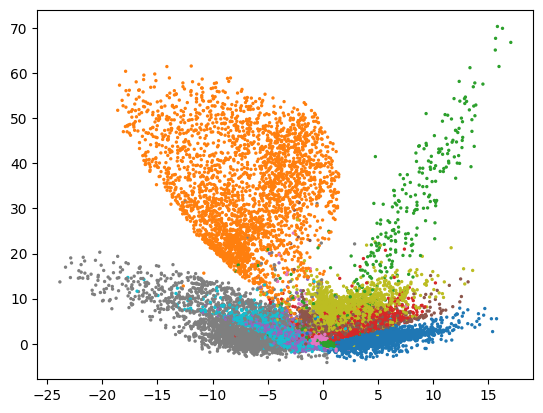
\includegraphics[scale=0.36]{img/mnist_latent.png}
      \caption{Training an autoencoder on MNIST and then visualizing the encodings from a 2D latent space shows the formation of distinct clusters, but there are huge empty spaces where the labeling may be ambiguous and not allow us to interpolate effectively. }
      \label{fig:mnist_latent}
    \end{subfigure}
    \hfill 
    \begin{subfigure}[b]{0.48\textwidth}
      \centering
      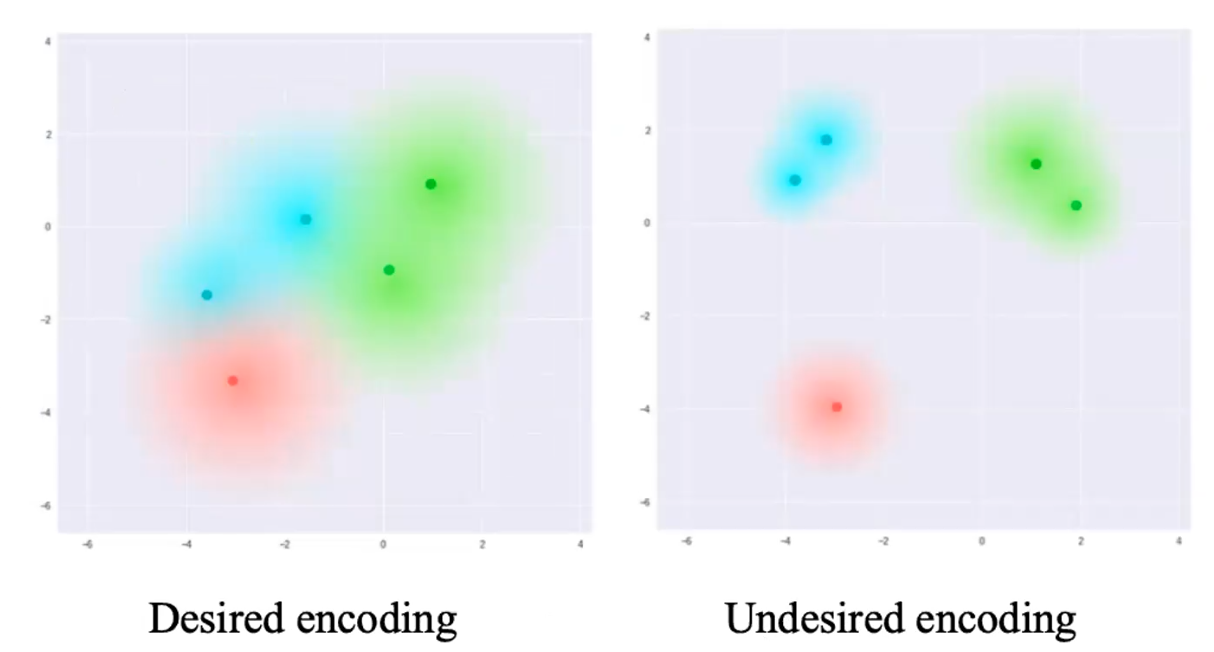
\includegraphics[scale=0.22]{img/contiguous_encoding.png}
      \caption{ Therefore, we want the encodings to be contiguous while still being distinct. This allows smooth interpolation which is easy to sample from with a simple pdf, e.g. Gaussian, and enables construction of \textit{new} samples. } 
      \label{fig:contiguous_encoding}
    \end{subfigure}
    \caption{}
    \label{fig:motivation_vae}
  \end{figure}

  In 2013, Kigma introduced this generative model that bridges between latent variable models and deep neural nets. We can think of the relationship between the linear model PCA and its latent counterpart PPCA as the relationship between the nonlinear autoencoders and variational autoencoders. This is a good time to review linear and nonlinear latent variable models in my ML notes. Note that in a LVM, the family of functions $\{D_\beta\}$ is used to map a latent variable $z$ to the likelihood $p(x \mid z)$. This can be done by a direct transformation of the random variable $Z$ (e.g. PPCA or as we will see later, \textit{normalizing flows}), or we can have $D_\beta(z)$ be an explicit parameterization (e.g. Gaussian mixture models and variational autoencoders). Given neural networks, we can do the latter method quite easily, and we are already familiar with the architectures to do so. 

  \begin{example}[Classification Nets Parameterize Multinomials]
    In a classification neural network with parameters $\beta$, it takes in an input $x$ and outputs a softmax vector $f_\beta (x) =(p_1, \ldots, p_K)^T$. This basically means that $f_\beta (x) = \theta$ parameterizes the conditional distribution (in this case, multinomial) of $y$ given $x$. 
    \begin{equation}
      Y \mid X = x \sim \mathrm{Multinomial}(\theta = f_\beta (x))
    \end{equation}
    This is a much more efficient way to store conditional distributions than a $\dim(X) (K - 1)$ lookup table. 
  \end{example}

  Therefore, by generating a latent variable $p(z)$ (that is simple and fixed), we can use a deep neural network $D_\beta$ to generate $\theta = D_\beta (z)$ which serve as the parameters of the conditional distribution $p_\theta (x \mid z)$, and then sampling from this distribution is easy because we assume that $p_\theta (x \mid z)$ is in an explicitly parameterized family of distributions. This allows us to easily sample from the joint distribution. 
  \begin{equation}
    p_\theta (x, z) = p_\theta (x \mid z) \, p(z)
  \end{equation}
  This is all great, but computing 
  \begin{equation}
    p(x) = \int p(x, z) \,dz = \int p_\theta (x \mid z) \, p(z) \,dz
  \end{equation}
  is computationally intractable. With strong assumptions, like conditional independence of not just $p(x \mid z)$ but \textit{also} $p(z \mid x)$, in RBMs, we can construct pretty good approximations. Recall that for RBMs, the derivative of the log of $p(x)$ decomposes into a positive phase that requires you to integrate over $p(z \mid x)$, which is easy, and $p(x, h)$, which is hard to do in general. But through contrastive divergence, we can approximate the integral by sampling a $\Tilde{x}$ and constructing another integral over $p(z \mid x)$, which is then easy to compute. 

  \begin{example}[Bernoulli-Bernoulli RBM] 
    We would like to approximate a $d$-dimensional Bernoulli vector $x$ with a latent variable $z \in \mathbb{R}^K$. We will assume a prior $p(z) \sim N(0, I)$, and let us have a neural net $D_{\beta}$ that parameterizes the random vector $x$, where $x_i \sim \mathrm{Bernoulli}(\theta_i)$ for $\theta_i$. Then, by conditional independence, 
    \begin{equation}
      p(x \mid z) = \prod_{i=1}^d p_\theta (x_i \mid z) = \prod_{i=1}^d \theta_i^{x_i} (1 - \theta_i)^{1 - x_i} = \prod_{i=1}^d \big[ D_\beta(z) \big]_i^{x_i} \big( 1 - [D_\beta(z)]_d \big)^{1 - x_i}
    \end{equation}
    and we can see that since $p$ has the flexibility of whatever vector in $[0, 1]^D$ it can be captured by the neural net $D_\beta$. It encompasses a broad family of Bernoulli probability distributions. We can see that we have some method to compute $p(x \mid z)$. We train a neural net (somehow) and do forward prop on it to generate the correct parameters modeling the distribution of $x$. Note that in RBMs the conditional independence allowed us to integrate over $z$ easily. To see why, in the example above, the integral becomes
    \begin{equation}
      p(x) = \sum_{z \in \{0, 1\}^k} \bigg\{ \prod_{i=1}^d \big[ D_\beta(z) \big]_i^{x_i} \big( 1 - [D_\beta(z)]_d \big)^{1 - x_i} \bigg\} p(z) 
    \end{equation}
    where $k$ is the dimension of the latent space. However, integrating over all $z$'s for more complex spaces is not feasible. 
  \end{example}

  $D_\beta$ is clearly nonlinear and we can't just do some simple closed form optimization, so we must use the tools introduced in nonlinear latent variable models. Namely, we revisit the variational lower bound. Recall that estimating the true $p(x)$ can be reduced to the problem of finding a good approximate of the true $p(z \mid x)$, the \textit{posterior} or \textit{inference component}, with some family of distributions $\{ q_\phi \}$. Just like the generation model, we can build another neural network $E_{\alpha}$ such that $\phi = E_{\alpha} (x)$ parameterizes the conditional distribution of $z$, called our \textit{encoder}. 
  \begin{equation}
    p(z \mid x) \approx q_\phi (z \mid x) = q_{E_\alpha (x)} (z)
  \end{equation}

  \begin{example}[Encoder Neural Net Generates Parameters of Likelihood]
    If $\phi = (\mu, \sigma)$, where $\sigma$ is just the vector representing variances of independent Gaussians, then we can use the neural network $E$ to get $\phi = E_{\alpha} (x)$. In the example, $\phi = (\mu, \log \sigma^2)$ since we want to allow negative values, and 
    \begin{equation}
      q_\phi (z \mid x) \sim \mathcal{N}(E_\alpha (x)) = \mathcal{N}(\phi) = \mathcal{N} (\mu, \sigma^2)
    \end{equation}
  \end{example} 

  Therefore, by modeling both the likelihood and posterior with probability distributions that can be parameterized by an output of neural networks, we have a \textit{variational autoencoder}. 

  \begin{definition}[Variational Autoencoders]
    In a \textbf{variational autoencoder (VAE)}, we assume that the covariates $x^{(i)} \sim X$ are generated as the marginal of a joint distribution $p(x, z)$ with latent variable $z \sim X$. We model the sub-distributions as such: 
    \begin{enumerate}
      \item We assume that the prior $p(z)$ is of fixed simple form, e.g. a standard Gaussian. 
      \item We assume that the likelihood $p(x \mid z)$ can be approximated by a parameteric family of distributions $p_\theta (x \mid z)$, where $\theta = D_\beta (z)$ is generated by a \textbf{decoder} neural network parameterized by $\beta$.
      \item We assume that the posterior $p(z \mid x)$ can be approximated by a parameteric family of distributions $q_\phi (z \mid x)$,\footnote{Note that this is an assumption! The posterior may be an arbitrary shape or form.} where $\phi = E_\alpha (x)$ is generated by an \textbf{encoder} neural network parameterized by $\alpha$.
    \end{enumerate} 
    We can optimize $\theta, \lambda$ by equivalently optimizing the parameters $\alpha, \beta$ of the nets. Once this is done, 
    \begin{enumerate}
      \item To conduct inference, we can input in some data $x$ and retrieve the distribution of its latent representation as $q_{E_\alpha (x)} \approx p (z \mid x)$. 
      \item To generate data, we can sample $z$ from $p(z)$ and sample from $p_{D_\beta (z)} (x) \approx p (x \mid z)$. 
    \end{enumerate}
  \end{definition} 

  \begin{figure}[H]
    \centering 
    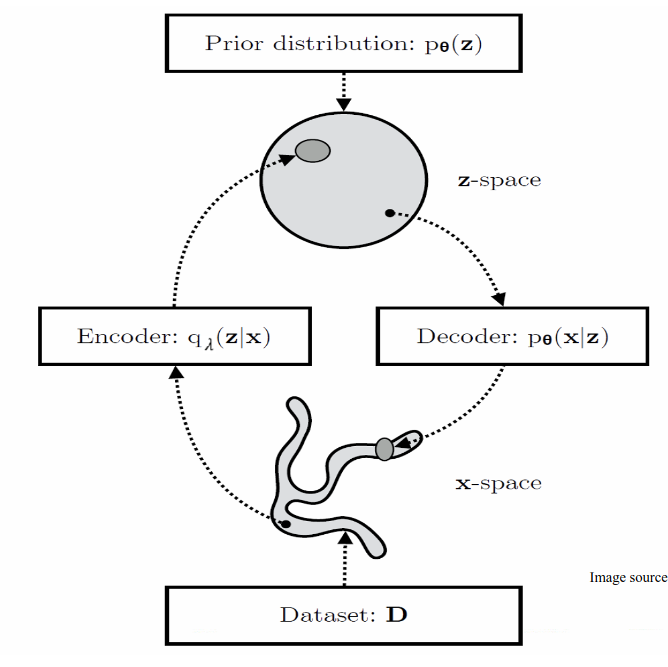
\includegraphics[scale=0.4]{img/VAE_framework.png}
    \caption{A pictorial diagram of a nonlinear latent variable model to refresh your memory.} 
    \label{fig:vae_framework}
  \end{figure}

  So how do we actually train this? Just like with every other nonlinear latent variable models, we can use the evidence lower bound. We do a quick review. Recall that the KL divergence can be decomposed into the sum of conditional entropies, and hence we can use the fact the KL divergence is always nonnegative to create this bound. 
  \begin{align}
    \log p_\theta (x) & = KL \big( q_\phi (z \mid x) \mid\mid p_{\theta} (z \mid x) \big) + \mathbb{E}_{q_{\phi} (z \mid x)} [\log p_{\theta} (x, z)] - \mathbb{E}_{q_\phi(z \mid x)} [ \log q_{\phi} (z \mid x)] \\
                      & \geq \mathbb{E}_{q_{\phi} (z \mid x)} [\log p_{\theta} (x, z)] - \mathbb{E}_{q_\phi(z \mid x)} [ \log q_{\phi} (z \mid x)] = \elbo(x, \phi, \theta)
  \end{align}
  and therefore by summing over all the data points we can get the evidence lower bound, which holds for any set of distributions $q_\phi^{(1)}, \ldots, q_\phi^{(N)}$.  
  \begin{equation}
    \sum_{i=1}^N \log p_{\theta} (x^{(i)}) \geq \sum_{i=1}^N \mathbb{E}_{q_\phi (z \mid x^{(i)})} [ \log p_{\theta} (x^{(i)}, z)] - \sum_{i=1}^N \mathbb{E}_{q_{\phi} (z \mid x^{(i)})} [ \log q_{\phi} (z \mid x^{(i)}) ] = \elbo(\mathcal{D}, \phi, \theta)
  \end{equation}
  Therefore, minimizing the KL divergence is equivalent to maximizing the ELBO w.r.t. $\theta$ and $\phi$. As we have seen in my ML notes, the gradient of the ELBO w.r.t. $\theta$ be solved by computing the gradient directly and using SGD. However, taking the gradient w.r.t. $\phi$ is more complicated since we cannot put the gradient in the expectation (since we are deriving and integrating w.r.t. $\phi$). We can use the log-derivative trick\footnote{explained in my ML notes}, but this is known to have high variance and is not sufficient to backpropagate huge neural nets. This is not actually the biggest problem either, as we will see that the extra parameters we've introduce with the neural nets do not allow us to backpropagate across stochastic variables. 

  Now we talk about more implementation details presented in the paper, which is a simplified form. 
  \begin{enumerate}
    \item The first is that \cite{vae} fixes a prior isotropic multivariate Gaussian $p_\theta (z) = \mathcal{N}(0, I)$, which lacks parameters. 

    \item It also assumes that $p_\theta (x \mid z)$ be a multivariate Gaussian (for real-valued data) or Bernoulli (in binary data). This gives us a nice parameteric form that may hopefully approximate the true posterior, which may be extremely complicated. 
    \begin{align}
      p_\theta (x \mid z) & = \mathcal{N}(\mu^{(i)}, \sigma^{2(i)} I) \qquad \theta = \{\mu^{(i)}, \sigma^{2 (i)} \} = D_\beta (z^{(i)}) \\
      p_\theta (x \mid z) & = \mathrm{Bernoulli}(\theta) \qquad \theta = D_\beta (z^{(i)}) 
    \end{align}

    \item It finally assumes that the true posterior $p_\theta (z \mid x)$, which is intractable, takes on a form $q_\phi (z \mid x)$ that can be approximated by a Gaussian with diagonal covariance. 
    \begin{equation}
      q_\phi (z \mid x^{(i)}) = \mathcal{N}(\mu^{(i)}, \sigma^{2 (i)} I) \qquad \phi = \{\mu^{(i)}, \sigma^{2 (i)} \} = E_\alpha (x^{(i)})
    \end{equation}
  \end{enumerate} 

  So let's walk through the forward propagation with the likelihood set to Bernoulli. We have a dataset $\{x^{(i)}\}$. For each $x^{(i)}$
  \begin{enumerate}
    \item We put it into our encoder network and get out the parameters $\phi^{(i)} = E_\alpha (x^{(i)})$ for our latent Gaussian. We output the mean $\mu_\alpha^{(i)}$ and either the variance $(\sigma_{\alpha}^{(i)})^2$, or the log-variance $\log (\sigma_{\alpha}^{(i)})^2$.\footnote{Since variances must always be positive, sometimes a slight tweaking of transformations is needed. For example, if an encoder network has a final linear layer, then the variances may not be always positive, which is a problem, so we may do an exponential or a ReLU at the end. You may notice that the log may often return negative numbers, but as we will see later, we can add a corresponding transformation in our \textit{reparamaterization trick}, which will exponentiate the log-variances (this is how it's implemented in the code) before using them as variances. Calculating the log-variance first and then exponentiating it may also bring better numerical stability.}

    \item We sample a $z^{(i)}$ from this Gaussian and feed it into the decoder network $D_\beta(z^{(i)})$, which returns the parameters $\theta^{(i)} = D_\beta (z^{(i)})$ for our Bernoulli likelihood. 

    \item We sample $\hat{x}^{(i)}$ from this Bernoulli and retrieve another sampled version of our input. 
  \end{enumerate} 

  Great, so we can draw a computation graph for this, but before we do, let's revisit the basics and draw a simpler example. 

  \begin{example}[Softmax]
    In the graph below, note that our ``prediction'' $\hat{y}^{(i)}$ for the data point $x^{(i)}$ is not really a prediction at all. If we have three categories (cat, dog, fish) and I give you an image, the model will output a vector of probabilities, e.g. $\hat{y}^{(i)} = [0.1, 0.2, 0.7]$. While we can easily infer that the probability of a fish is highest, and therefore should be our prediction, the model didn't actually output one answer. Rather, we should interpret this output vector $\hat{y}^{(i)}$ as a \textit{parameter} $\theta$ of a multinomial distribution. From this we can \textit{sample} an actual prediction $\hat{y}^{(i)} \sim \mathrm{Multinomial}(\theta)$. 

    When we compute the loss of a sample, we compute the likelihood by taking the true output $y^{(i)}$ and one-hot encoding it. One-hot encoding allows us to convert the label $y^{(i)}$ into a parameter of a multinomial itself, and this process is hidden inside $\ell$. Therefore we want to maximize
    \begin{equation}
      \log p(y^{(i)} \mid x^{(i)}) = p_{\hat{\theta^{(i)}}} (y^{(i)}) = \sum_j y_j^{(i)} \log  \hat{\theta}^{(i)}_j 
    \end{equation}
    which is the cross entropy. 

    \begin{figure}[H]
      \centering
      \tikzset{every picture/.style={line width=0.75pt}} %set default line width to 0.75pt        
      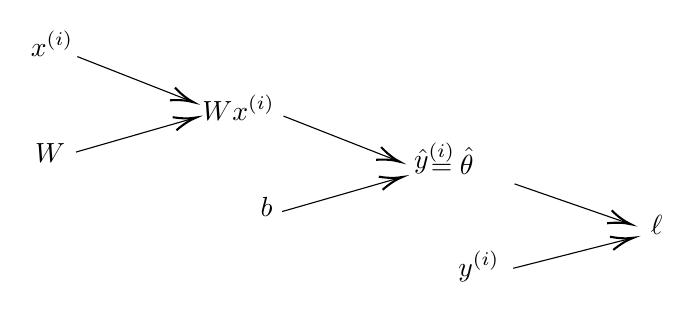
\begin{tikzpicture}[x=0.75pt,y=0.75pt,yscale=-1,xscale=1]
        %uncomment if require: \path (0,203); %set diagram left start at 0, and has height of 203

        %Straight Lines [id:da7538339934106768] 
        \draw    (267,80.33) -- (321.14,101.6) ;
        \draw [shift={(323,102.33)}, rotate = 201.45] [color={rgb, 255:red, 0; green, 0; blue, 0 }  ][line width=0.75]    (10.93,-3.29) .. controls (6.95,-1.4) and (3.31,-0.3) .. (0,0) .. controls (3.31,0.3) and (6.95,1.4) .. (10.93,3.29)   ;
        %Straight Lines [id:da025730723330035343] 
        \draw    (266.33,126.33) -- (322.41,110.22) ;
        \draw [shift={(324.33,109.67)}, rotate = 163.97] [color={rgb, 255:red, 0; green, 0; blue, 0 }  ][line width=0.75]    (10.93,-3.29) .. controls (6.95,-1.4) and (3.31,-0.3) .. (0,0) .. controls (3.31,0.3) and (6.95,1.4) .. (10.93,3.29)   ;
        %Straight Lines [id:da6718586456674974] 
        \draw    (378.33,113) -- (432.44,131.79) ;
        \draw [shift={(434.33,132.45)}, rotate = 199.15] [color={rgb, 255:red, 0; green, 0; blue, 0 }  ][line width=0.75]    (10.93,-3.29) .. controls (6.95,-1.4) and (3.31,-0.3) .. (0,0) .. controls (3.31,0.3) and (6.95,1.4) .. (10.93,3.29)   ;
        %Straight Lines [id:da7837038799068268] 
        \draw    (377.67,153.67) -- (433.73,139.42) ;
        \draw [shift={(435.67,138.93)}, rotate = 165.75] [color={rgb, 255:red, 0; green, 0; blue, 0 }  ][line width=0.75]    (10.93,-3.29) .. controls (6.95,-1.4) and (3.31,-0.3) .. (0,0) .. controls (3.31,0.3) and (6.95,1.4) .. (10.93,3.29)   ;
        %Straight Lines [id:da686511913498152] 
        \draw    (167.67,51.67) -- (221.81,72.94) ;
        \draw [shift={(223.67,73.67)}, rotate = 201.45] [color={rgb, 255:red, 0; green, 0; blue, 0 }  ][line width=0.75]    (10.93,-3.29) .. controls (6.95,-1.4) and (3.31,-0.3) .. (0,0) .. controls (3.31,0.3) and (6.95,1.4) .. (10.93,3.29)   ;
        %Straight Lines [id:da9460066058545258] 
        \draw    (167,97.67) -- (223.08,81.55) ;
        \draw [shift={(225,81)}, rotate = 163.97] [color={rgb, 255:red, 0; green, 0; blue, 0 }  ][line width=0.75]    (10.93,-3.29) .. controls (6.95,-1.4) and (3.31,-0.3) .. (0,0) .. controls (3.31,0.3) and (6.95,1.4) .. (10.93,3.29)   ;

        % Text Node
        \draw (144,38) node [anchor=north west][inner sep=0.75pt]   [align=left] {$\displaystyle x^{( i)}$};
        % Text Node
        \draw (146,92.33) node [anchor=north west][inner sep=0.75pt]   [align=left] {$\displaystyle W$};
        % Text Node
        \draw (226.67,68.67) node [anchor=north west][inner sep=0.75pt]   [align=left] {$\displaystyle Wx^{( i)}$};
        % Text Node
        \draw (254.67,118.33) node [anchor=north west][inner sep=0.75pt]   [align=left] {$\displaystyle b$};
        % Text Node
        \draw (328.67,92) node [anchor=north west][inner sep=0.75pt]   [align=left] {$\displaystyle \hat{y}^{( i)}$};
        % Text Node
        \draw (350,144) node [anchor=north west][inner sep=0.75pt]   [align=left] {$\displaystyle y^{( i)}$};
        % Text Node
        \draw (442.67,127) node [anchor=north west][inner sep=0.75pt]   [align=left] {$\displaystyle \ell $};
        % Text Node
        \draw (336.67,94.33) node [anchor=north west][inner sep=0.75pt]   [align=left] {$\displaystyle =\hat{\theta }$};
      \end{tikzpicture}
      \caption{ When we draw a computation graph to visualize the backpropagation of a softmax regression function, note that we need to have the gradients start from the log-likelihood $\ell$ and reach ``back'' to $W$ and $b$, our model parameters. }
      \label{fig:softmax1}
    \end{figure}

    Another way to approximate the log likelihood $\ell$ is to simply take the output parameter $\hat{\theta}^{(i)}$, keep on sampling $y$'s from it, penalizing when needed, and averaging the penalties.\footnote{This is useful if we can easily sample, but do not know the closed form of the likelihood distribution.}
    \begin{align}
      \log p(y^{(i)} \mid x^{(i)}) & = \log \mathbb{E}_{y \sim \hat{\theta}^{(i)}} \big[ \mathbbm{1}_{y^{i} = y} \big] \\
                                   & = \log \int \mathbbm{1}_{y^{(i)} = y} p_{\hat{\theta}^{(i)}} (y) \,dy \\
                                   & \approx \log \bigg\{ \frac{1}{N} \sum_{l=1}^L \mathbbm{1}_{y^{(i)} = y^{(i, l)}} \bigg\}
    \end{align}
    where $y^{(i, l)} \sim \mathrm{Multinomial} (\hat{\theta}^{(i)})$. 

    \begin{figure}[H]
      \centering
      \tikzset{every picture/.style={line width=0.75pt}} %set default line width to 0.75pt        
      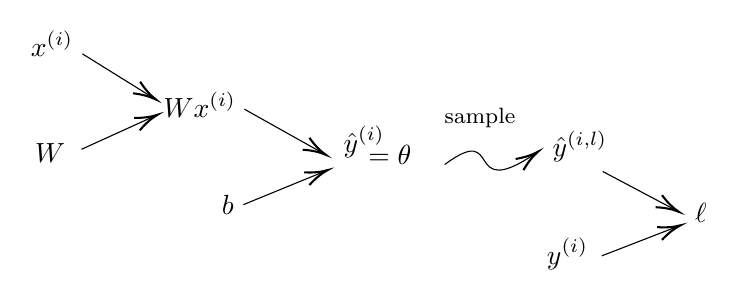
\begin{tikzpicture}[x=0.75pt,y=0.75pt,yscale=-1,xscale=1]
        %Straight Lines [id:da7816088828640423] 
        \draw    (221.47,81) -- (258.99,102.02) ;
        \draw [shift={(260.73,103)}, rotate = 209.26] [color={rgb, 255:red, 0; green, 0; blue, 0 }  ][line width=0.75]    (10.93,-3.29) .. controls (6.95,-1.4) and (3.31,-0.3) .. (0,0) .. controls (3.31,0.3) and (6.95,1.4) .. (10.93,3.29)   ;
        %Straight Lines [id:da936006232356312] 
        \draw    (221,127) -- (259.82,111.09) ;
        \draw [shift={(261.67,110.33)}, rotate = 157.71] [color={rgb, 255:red, 0; green, 0; blue, 0 }  ][line width=0.75]    (10.93,-3.29) .. controls (6.95,-1.4) and (3.31,-0.3) .. (0,0) .. controls (3.31,0.3) and (6.95,1.4) .. (10.93,3.29)   ;
        %Straight Lines [id:da6326384434909695] 
        \draw    (394.1,111) -- (429.03,129.51) ;
        \draw [shift={(430.79,130.45)}, rotate = 207.93] [color={rgb, 255:red, 0; green, 0; blue, 0 }  ][line width=0.75]    (10.93,-3.29) .. controls (6.95,-1.4) and (3.31,-0.3) .. (0,0) .. controls (3.31,0.3) and (6.95,1.4) .. (10.93,3.29)   ;
        %Straight Lines [id:da06163876606511509] 
        \draw    (393.67,151.67) -- (429.8,137.66) ;
        \draw [shift={(431.67,136.93)}, rotate = 158.81] [color={rgb, 255:red, 0; green, 0; blue, 0 }  ][line width=0.75]    (10.93,-3.29) .. controls (6.95,-1.4) and (3.31,-0.3) .. (0,0) .. controls (3.31,0.3) and (6.95,1.4) .. (10.93,3.29)   ;
        %Straight Lines [id:da9024565670445639] 
        \draw    (143.42,54.33) -- (177.13,75.28) ;
        \draw [shift={(178.82,76.33)}, rotate = 211.86] [color={rgb, 255:red, 0; green, 0; blue, 0 }  ][line width=0.75]    (10.93,-3.29) .. controls (6.95,-1.4) and (3.31,-0.3) .. (0,0) .. controls (3.31,0.3) and (6.95,1.4) .. (10.93,3.29)   ;
        %Straight Lines [id:da5276819560809279] 
        \draw    (143,100.33) -- (177.85,84.49) ;
        \draw [shift={(179.67,83.67)}, rotate = 155.56] [color={rgb, 255:red, 0; green, 0; blue, 0 }  ][line width=0.75]    (10.93,-3.29) .. controls (6.95,-1.4) and (3.31,-0.3) .. (0,0) .. controls (3.31,0.3) and (6.95,1.4) .. (10.93,3.29)   ;
        %Curve Lines [id:da9806340335414951] 
        \draw    (318,107.67) .. controls (346.57,86.43) and (326.3,126.22) .. (361.36,102.57) ;
        \draw [shift={(363,101.44)}, rotate = 145.15] [color={rgb, 255:red, 0; green, 0; blue, 0 }  ][line width=0.75]    (10.93,-3.29) .. controls (6.95,-1.4) and (3.31,-0.3) .. (0,0) .. controls (3.31,0.3) and (6.95,1.4) .. (10.93,3.29)   ;

        % Text Node
        \draw (117.33,42) node [anchor=north west][inner sep=0.75pt]   [align=left] {$\displaystyle x^{( i)}$};
        % Text Node
        \draw (119.33,96.33) node [anchor=north west][inner sep=0.75pt]   [align=left] {$\displaystyle W$};
        % Text Node
        \draw (181.33,71.33) node [anchor=north west][inner sep=0.75pt]   [align=left] {$\displaystyle Wx^{( i)}$};
        % Text Node
        \draw (209.33,121) node [anchor=north west][inner sep=0.75pt]   [align=left] {$\displaystyle b$};
        % Text Node
        \draw (268,88) node [anchor=north west][inner sep=0.75pt]   [align=left] {$\displaystyle \hat{y}^{( i)}$};
        % Text Node
        \draw (366,142) node [anchor=north west][inner sep=0.75pt]   [align=left] {$\displaystyle y^{( i)}$};
        % Text Node
        \draw (437.33,125) node [anchor=north west][inner sep=0.75pt]   [align=left] {$\displaystyle \ell $};
        % Text Node
        \draw (280,97) node [anchor=north west][inner sep=0.75pt]   [align=left] {$\displaystyle =\theta $};
        % Text Node
        \draw (316.67,79) node [anchor=north west][inner sep=0.75pt]  [font=\footnotesize] [align=left] {$\displaystyle \text{\text{sample}}$};
        % Text Node
        \draw (368.67,90) node [anchor=north west][inner sep=0.75pt]   [align=left] {$\displaystyle \hat{y}^{( i,l)}$};
      \end{tikzpicture}
      \caption{Note that since it's much harder to sample and converge onto a good approximation, it's tougher to go through the curly arrow. That is, it is harder to backpropagate through \textbf{stochastic nodes}. }
      \label{fig:softmax2}
    \end{figure}

    Therefore, we can think of backpropagating as either one of two things. Either backpropagate straight through the parameter like we did first, or sample from the estimated distribution and sum up to approximate the samples. 
  \end{example}

  Let's keep this in the back of our mind, and focus on the computation for a bit. By the simplifying form that $q_\phi$ is a Gaussian, we can even get a nearly closed form of the ELBO. 

  \begin{theorem}
    Given the assumptions above, 
    \begin{align}
      \elbo(x, \phi, \theta) & \coloneqq \mathbb{E}_{q_\phi(z \mid x)} [ \log p_\theta (x \mid z)] + \mathbb{E}_{q_\phi (z \mid x)} [ \log p(z)] - \mathbb{E}_{q_\phi (z \mid x)} [ \log q_\phi (z \mid x)] \\
                             & = \mathbb{E}_{q_\phi(z \mid x)} [ \log p_\theta (x \mid z)] + \frac{1}{2} \sum_{d=1}^D \bigg( 1 + \log( (\sigma_d)^2 ) - (\mu_d)^2 - (\sigma_d)^2 \bigg)
    \end{align}
    Therefore, the derivative of last two terms are \textit{exact}, i.e. we don't need to estimate them with SGD. 
  \end{theorem}
  \begin{proof}
    Let's evaluate the last two expectations. 
    \begin{align}
      \mathbb{E}_{q_\phi (z \mid x)} [ \log p(z)] & = \int \log p(z) \cdot q_\phi (z \mid x) \,dx \\
                                                  & = \int \log \{\mathcal{N} (z \mid 0, I) \}  \cdot \mathcal{N}(z \mid \mu, \sigma^2) \,dz  \\
                                                  & = - \frac{D}{2} \log (2 \pi) - \frac{1}{2} \sum_{d=1}^D \mu_d^2 + \sigma_d^2) \\
      \mathbb{E}_{q_\phi (z \mid x)} [ \log q_\phi (z \mid x)] & = \int \log q_\phi (z \mid x) \, q_\phi (z \mid x) \,dz \\
                                                               & = \int \log \{ \mathcal{N}(z \mid \mu, \sigma^2) \} \mathcal{N}(z \mid \mu, \sigma^2) \,dx \\
                                                               & = -\frac{D}{2} \sum_{d=1}^D 1 + \log (\sigma_d^2)
    \end{align}
  \end{proof} 

  \begin{corollary}[Bernoulli Likelihood]
    If $p\theta (x \mid z)$ is Bernoulli, then the ELBO can be estimated by estimating the likelihood 
    \begin{equation}
      \elbo(x, \phi, \theta) = \frac{1}{L} \sum_{l=1}^L + \frac{1}{2} \sum_{d=1}^D \bigg( 1 + \log( (\sigma_d)^2 ) - (\mu_d)^2 - (\sigma_d)^2 \bigg)
    \end{equation}
  \end{corollary}


  With these two things, let's take a look at the computation graph of the VAE. 

  \begin{figure}[H]
    \centering 
    \tikzset{every picture/.style={line width=0.75pt}} %set default line width to 0.75pt        
    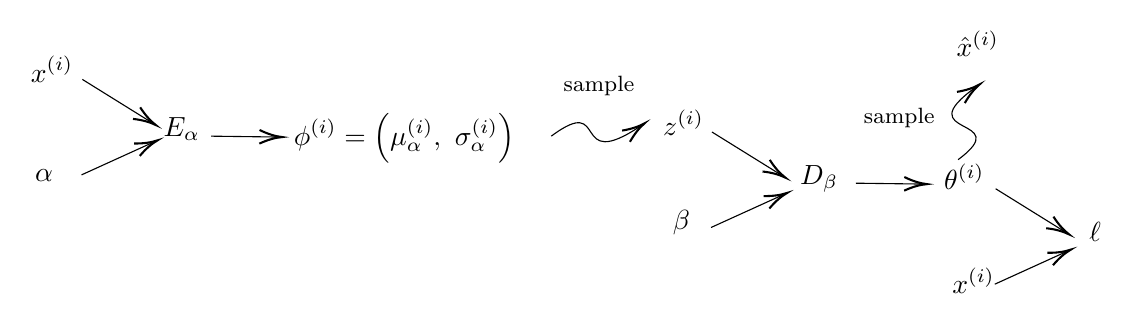
\begin{tikzpicture}[x=0.75pt,y=0.75pt,yscale=-1,xscale=1]
      %uncomment if require: \path (0,160); %set diagram left start at 0, and has height of 160

      %Straight Lines [id:da549284335951172] 
      \draw    (68.09,34.33) -- (101.79,55.28) ;
      \draw [shift={(103.49,56.33)}, rotate = 211.86] [color={rgb, 255:red, 0; green, 0; blue, 0 }  ][line width=0.75]    (10.93,-3.29) .. controls (6.95,-1.4) and (3.31,-0.3) .. (0,0) .. controls (3.31,0.3) and (6.95,1.4) .. (10.93,3.29)   ;
      %Straight Lines [id:da6162521420944999] 
      \draw    (67.67,80.33) -- (102.51,64.49) ;
      \draw [shift={(104.33,63.67)}, rotate = 155.56] [color={rgb, 255:red, 0; green, 0; blue, 0 }  ][line width=0.75]    (10.93,-3.29) .. controls (6.95,-1.4) and (3.31,-0.3) .. (0,0) .. controls (3.31,0.3) and (6.95,1.4) .. (10.93,3.29)   ;
      %Straight Lines [id:da12977974645980606] 
      \draw    (130.09,61.67) -- (162.33,62.09) ;
      \draw [shift={(164.33,62.11)}, rotate = 180.74] [color={rgb, 255:red, 0; green, 0; blue, 0 }  ][line width=0.75]    (10.93,-3.29) .. controls (6.95,-1.4) and (3.31,-0.3) .. (0,0) .. controls (3.31,0.3) and (6.95,1.4) .. (10.93,3.29)   ;
      %Curve Lines [id:da5962854824857341] 
      \draw    (294,61.67) .. controls (322.57,40.43) and (302.3,80.22) .. (337.36,56.57) ;
      \draw [shift={(339,55.44)}, rotate = 145.15] [color={rgb, 255:red, 0; green, 0; blue, 0 }  ][line width=0.75]    (10.93,-3.29) .. controls (6.95,-1.4) and (3.31,-0.3) .. (0,0) .. controls (3.31,0.3) and (6.95,1.4) .. (10.93,3.29)   ;
      %Straight Lines [id:da19986172160423643] 
      \draw    (371.42,59.67) -- (405.13,80.61) ;
      \draw [shift={(406.82,81.67)}, rotate = 211.86] [color={rgb, 255:red, 0; green, 0; blue, 0 }  ][line width=0.75]    (10.93,-3.29) .. controls (6.95,-1.4) and (3.31,-0.3) .. (0,0) .. controls (3.31,0.3) and (6.95,1.4) .. (10.93,3.29)   ;
      %Straight Lines [id:da563527517377988] 
      \draw    (371,105.67) -- (405.85,89.83) ;
      \draw [shift={(407.67,89)}, rotate = 155.56] [color={rgb, 255:red, 0; green, 0; blue, 0 }  ][line width=0.75]    (10.93,-3.29) .. controls (6.95,-1.4) and (3.31,-0.3) .. (0,0) .. controls (3.31,0.3) and (6.95,1.4) .. (10.93,3.29)   ;
      %Straight Lines [id:da9810030545590435] 
      \draw    (440.75,84.33) -- (473,84.75) ;
      \draw [shift={(475,84.78)}, rotate = 180.74] [color={rgb, 255:red, 0; green, 0; blue, 0 }  ][line width=0.75]    (10.93,-3.29) .. controls (6.95,-1.4) and (3.31,-0.3) .. (0,0) .. controls (3.31,0.3) and (6.95,1.4) .. (10.93,3.29)   ;
      %Curve Lines [id:da27917860120610793] 
      \draw    (490,73) .. controls (518.57,51.77) and (464.66,62.45) .. (498.72,37.92) ;
      \draw [shift={(500.33,36.78)}, rotate = 145.15] [color={rgb, 255:red, 0; green, 0; blue, 0 }  ][line width=0.75]    (10.93,-3.29) .. controls (6.95,-1.4) and (3.31,-0.3) .. (0,0) .. controls (3.31,0.3) and (6.95,1.4) .. (10.93,3.29)   ;
      %Straight Lines [id:da46048578655946304] 
      \draw    (508.09,87) -- (541.79,107.94) ;
      \draw [shift={(543.49,109)}, rotate = 211.86] [color={rgb, 255:red, 0; green, 0; blue, 0 }  ][line width=0.75]    (10.93,-3.29) .. controls (6.95,-1.4) and (3.31,-0.3) .. (0,0) .. controls (3.31,0.3) and (6.95,1.4) .. (10.93,3.29)   ;
      %Straight Lines [id:da4526948376904725] 
      \draw    (507.67,133) -- (542.51,117.16) ;
      \draw [shift={(544.33,116.33)}, rotate = 155.56] [color={rgb, 255:red, 0; green, 0; blue, 0 }  ][line width=0.75]    (10.93,-3.29) .. controls (6.95,-1.4) and (3.31,-0.3) .. (0,0) .. controls (3.31,0.3) and (6.95,1.4) .. (10.93,3.29)   ;

      % Text Node
      \draw (42,22) node [anchor=north west][inner sep=0.75pt]   [align=left] {$\displaystyle x^{( i)}$};
      % Text Node
      \draw (44,76.33) node [anchor=north west][inner sep=0.75pt]   [align=left] {$\displaystyle \alpha $};
      % Text Node
      \draw (106,51.33) node [anchor=north west][inner sep=0.75pt]   [align=left] {$\displaystyle E_{\alpha }$};
      % Text Node
      \draw (168.67,49.33) node [anchor=north west][inner sep=0.75pt]   [align=left] {$\displaystyle \phi ^{( i)} =\left( \mu _{\alpha }^{( i)} ,\ \sigma _{\alpha }^{( i)}\right)$};
      % Text Node
      \draw (298.67,31.67) node [anchor=north west][inner sep=0.75pt]  [font=\footnotesize] [align=left] {$\displaystyle \text{\text{sample}}$};
      % Text Node
      \draw (346.67,47.67) node [anchor=north west][inner sep=0.75pt]   [align=left] {$\displaystyle z^{( i)}$};
      % Text Node
      \draw (351.33,96.33) node [anchor=north west][inner sep=0.75pt]   [align=left] {$\displaystyle \beta $};
      % Text Node
      \draw (412.67,74.67) node [anchor=north west][inner sep=0.75pt]   [align=left] {$\displaystyle D_{\beta }$};
      % Text Node
      \draw (482,73.67) node [anchor=north west][inner sep=0.75pt]   [align=left] {$\displaystyle \theta ^{( i)}$};
      % Text Node
      \draw (443.33,47) node [anchor=north west][inner sep=0.75pt]  [font=\footnotesize] [align=left] {$\displaystyle \text{\text{sample}}$};
      % Text Node
      \draw (488,9.67) node [anchor=north west][inner sep=0.75pt]   [align=left] {$\displaystyle \hat{x}^{( i)}$};
      % Text Node
      \draw (486,123.67) node [anchor=north west][inner sep=0.75pt]   [align=left] {$\displaystyle x^{( i)}$};
      % Text Node
      \draw (552,101.67) node [anchor=north west][inner sep=0.75pt]   [align=left] {$\displaystyle \ell $};
    \end{tikzpicture}
    \caption{Computational graph of a VAE.} 
    \label{fig:vae_comp1}
  \end{figure}

  Note that since we have shown that the derivative of the last two expectations (i.e. the derivative of the KL divergence) is dependent on the outputs $\sigma$ and $\mu$ of the neural net, we must also backpropagate amongst them as well, which is why you see the giant arrow from $\phi$ to $\ell$. 

  We can see that since we know the closed form of $p_\theta (x \mid z)$, backpropagating over $\theta^{(i)}$ is no problem. However, we must reach $\alpha$ to update the neural network weights, and to do this we must go backprop through the stochastic node $z^{(i)}$, which may stump you. In fact, how do you even backpropagate against something that's a random variable? Remember that in our softmax example, we could simply compute the log likelihood of a bunch of samples at this node to get an approximate average log likelihood. This is a start, but in this case we want to compute the \textit{gradient} of the log likelihood. Fortunately, the \textit{log-derivative trick}\footnote{Mentioned in my ML notes} allows us to swap the gradient and expectation under a certain form, putting the expectation on the outside and therefore allowing us to sample gradients. 
  \begin{equation}
    \nabla_\phi \mathbb{E}_{q_\phi (z)} [f(z)] = \mathbb{E}_{q_\phi (z)} [ f(z) \nabla_\phi \log q_{\phi} (z)]
  \end{equation}

  So we apply the same idea by sampling $z^{(1)}, \ldots, z^{(L)}$ from the Gaussian with parameters $\phi^{(i)}$ and for each sample we fix $z^{(l)}$, allowing us to backpropagate to $\alpha$ to get a noisy estimate. By averaging these noisy gradients we have an approximation of the true gradient w.r.t. $x^{(i)}$.\footnote{This like a SGD inside a SGD, since we're sampling over minibatches of the samples $x^{(i)}$ as well.} Unfortunately, when doing this for gradients the variance tends to be very high up to a point where it is impractical, and even with a lot of sampling this frequently undershoots or overshoots the actual gradient. Therefore, we must come up with an alternative solution to estimate the gradient efficiently. 

\subsection{Reparamaterization Trick} 

  In 2013, Durk Kigma, then a PhD student in machine learning at the University of Amsterdam, introduced a solution in \cite{vae} called the \textit{reparamaterization trick}, which is just an application of a change of basis. 

  \begin{theorem}[Reparameterization Trick]
    Let $q_\phi(z|x)$ be a continuous distribution that can be sampled by first sampling $\epsilon \sim p(\epsilon)$ from a parameter-free distribution and then applying a differentiable transformation $g_\phi(\epsilon, x)$. Then:
    \begin{equation}
       \nabla_\phi \mathbb{E}_{q_\phi(z|x)} [f(z)] = \nabla_\phi \mathbb{E}_{p(\epsilon)} [f(g_\phi(\epsilon, x))] = \mathbb{E}_{p(\epsilon)} [\nabla_\phi f(g_\phi(\epsilon, x))] 
     \end{equation}
    or in integrals, 
    \begin{equation}
     \nabla_\phi \int f(z) \, q_\phi (z \mid x) \,dz = \nabla_\phi \int f(g_\phi (\epsilon, x)) \, p(\epsilon) \,d\epsilon = \int \nabla_\phi f(g_\phi (\epsilon, x)) \, p(\epsilon) \, d\epsilon 
    \end{equation}
    where $f$ is any differentiable function. 
  \end{theorem}
  \begin{proof}
    We clearly state our assumptions:
    \begin{itemize}
      \item We have a distribution $q_\phi(z|x)$ that can be reparameterized using $g_\phi(\epsilon, x)$
      \item $\epsilon$ is sampled from a parameter-free distribution $p(\epsilon)$
      \item $g_\phi$ is differentiable with respect to $\phi$
      \item $f$ is any differentiable function
    \end{itemize}

    The first equality to prove is:
    \begin{equation*}
        \nabla_\phi \mathbb{E}_{q_\phi(z|x)} [f(z)] = \nabla_\phi \mathbb{E}_{p(\epsilon)} [f(g_\phi(\epsilon, x))]
    \end{equation*}

    This follows directly from the reparameterization property. Since $z = g_\phi(\epsilon, x)$ where $\epsilon \sim p(\epsilon)$, we can rewrite any expectation over $q_\phi(z|x)$ as an expectation over $p(\epsilon)$:
    \begin{equation*}
        \mathbb{E}_{q_\phi(z|x)} [f(z)] = \mathbb{E}_{p(\epsilon)} [f(g_\phi(\epsilon, x))]
    \end{equation*}

    Taking $\nabla_\phi$ of both sides gives us the first equality. The second equality to prove is:
    \begin{equation}
      \nabla_\phi \mathbb{E}_{p(\epsilon)} [f(g_\phi(\epsilon, x))] = \mathbb{E}_{p(\epsilon)} [\nabla_\phi f(g_\phi(\epsilon, x))] \iff \nabla_\phi \int f(g_\phi(\epsilon, x)) p(\epsilon) d\epsilon = \int \nabla_\phi f(g_\phi(\epsilon, x)) p(\epsilon) d\epsilon
    \end{equation}

    To justify exchanging the gradient and integral, we invoke the Leibniz integral rule. This exchange is valid when $f \circ g_\phi$ is differentiable with respect to $\phi$ (given in our assumptions), the domain of integration (support of $p(\epsilon)$) is independent of $\phi$, and there are suitable integrability conditions (which we assume hold). Then we exchange the gradient and expectation:
    \begin{equation}
      \nabla_\phi \int f(g_\phi(\epsilon, x)) p(\epsilon) d\epsilon = \int \nabla_\phi f(g_\phi(\epsilon, x)) p(\epsilon) d\epsilon
    \end{equation}

    A crucial observation is that $p(\epsilon)$ does not depend on $\phi$ (it is parameter-free), which is essential for this exchange to work.
    \begin{equation}
        \nabla_\phi \mathbb{E}_{q_\phi(z|x)} [f(z)] = \nabla_\phi \mathbb{E}_{p(\epsilon)} [f(g_\phi(\epsilon, x))] = \mathbb{E}_{p(\epsilon)} [\nabla_\phi f(g_\phi(\epsilon, x))]
    \end{equation}
  \end{proof}

  This result is fundamental to variational inference and deep learning, particularly in training Variational Autoencoders (VAEs). The key insight is that by reparameterizing the random variable $z$ in terms of a parameter-free random variable $\epsilon$, we can separate the stochastic sampling (which is not differentiable) from the deterministic transformation $g_\phi$ (which is differentiable).

  The biggest advantage to this is that we although we do not avoid sampling to approximate the log likelihood, the rate at which it converges is much faster than simple sampling or the log-derivative trick, which is demonstrated in the example below. 

  \begin{example}[Gradient of Expection of $f(x) = x^2$ w.r.t. Gaussian]
    Assume we have a normal distribution $q$ that is parameterized by $\phi$, specifically
    $q_\phi(x) = N(\phi, 1)$. We want to solve the below problem
    \begin{equation}
      \min_\phi \mathbb{E}_q[x^2]
    \end{equation}

    This is of course a rather silly problem and the optimal $\phi = 0$ is obvious. One way to calculate $\nabla_\phi \mathbb{E}[x^2]$ is using the log-derivative trick as follows
    \begin{align}
      \nabla_\phi \mathbb{E}_q[x^2] &= \nabla_\phi\int q_\phi(x)x^2dx \\
      &= \int x^2\nabla_\phi q_\phi(x)\frac{q_\phi(x)}{q_\phi(x)}dx \\
      &= \int q_\phi(x)\nabla_\phi\log q_\phi(x)x^2dx \\
      &= \mathbb{E}_q[x^2\nabla_\phi\log q_\phi(x)]
    \end{align}

    For our example where $q_\phi(x) = N(\phi, 1)$, this method gives
    \begin{equation}
      \nabla_\phi \mathbb{E}[x^2] = \mathbb{E}_q[x^2(x-\phi)]
    \end{equation}
    and we can sample from $q \sim N(\phi, 1)$. Reparameterization trick is a way to rewrite the expectation so that the distribution with respect to which we take the gradient is independent of parameter $\phi$. To achieve this, we need to make the stochastic element in $q$ independent of $\phi$. Hence, we write $x$ as
    \begin{equation}
      x = \phi+ \epsilon, \quad \epsilon \sim N(0,1)
    \end{equation}

    Then, we can write
    \begin{equation}
      \mathbb{E}_q[x^2] = \mathbb{E}_{\epsilon} [(\phi+ \epsilon)^2]
    \end{equation}

    where $p(\epsilon)$ is the distribution of $\epsilon$, i.e., $N(0,1)$. Now we can write the derivative of $\mathbb{E}_q[x^2]$ as
    follows
    \begin{equation}
      \nabla_\phi \mathbb{E}[x^2] = \nabla_\phi \mathbb{E}_p[(\phi+ \epsilon)^2] = \mathbb{E}_p[2(\phi+ \epsilon)]
    \end{equation}
    If we actually plot the variances, for sample sizes of $N = 10, 100, 1000, 10000, 100000$, we can see that the reparamaterization trick produces estimates where the variances of the sampling distribution is an order of magnitude smaller. 

    \begin{figure}[H]
      \centering 
      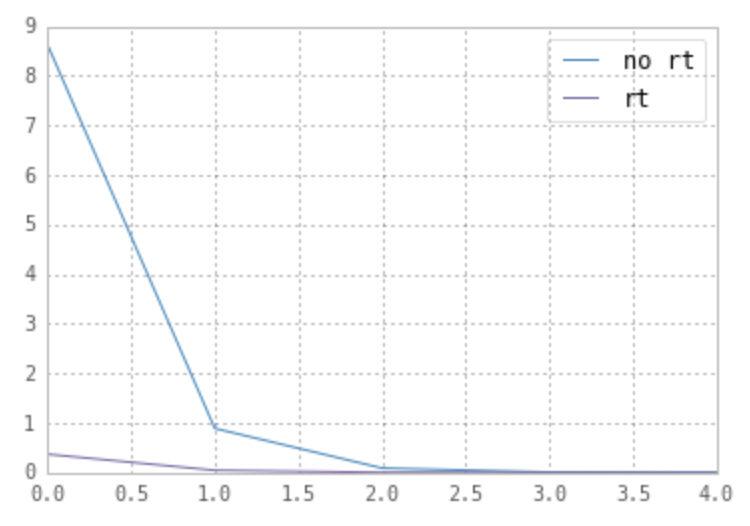
\includegraphics[scale=0.6]{img/reparam.png}
      \caption{Credits to \href{https://stats.stackexchange.com/questions/199605/how-does-the-reparameterization-trick-for-vaes-work-and-why-is-it-important}{here}.} 
      \label{fig:reparam}
    \end{figure}
  \end{example}

  Therefore, given that $\phi_\mu = \mu^{(i)}$ and $\phi_\sigma = (\sigma^{(i)})^2$ are the outputs of our encoder neural net, our transformation is 
  \begin{equation}
    g_\phi (x, \epsilon^{(l)}) = \phi_\mu + \sqrt{\phi_\sigma} \odot \epsilon^{(l)} = \mu^{(i)} + \sigma^{(i)} \odot \epsilon^{(l)} \qquad \epsilon^{(l)} \sim \mathcal{N}(0, I)
  \end{equation}
  or in the log-variance case, where the encoder outputs $\phi_\sigma = \log (\sigma^{(i)})^2 = 2 \log \sigma^{(i)}$, we have 
  \begin{equation}
    g_\phi (x, \epsilon^{(l)}) = \mu^{(i)} + e^{\phi_\sigma/2} \odot \epsilon^{(l)} = \mu^{(i)} + \sigma^{(i)} \odot \epsilon^{(l)} \qquad \epsilon^{(l)} \sim \mathcal{N}(0, I)
  \end{equation}

  where $\odot$ is element-wise multiplication, can be used to model $p(z)$.\footnote{This is called \textbf{factorized Gaussian posterior}, but it can be extended to the \textbf{full-variance Gaussian posterior} where the variance is parameterized through a lower triangular matrix $L$, from the Cholesky decomposition.} The intuition behind this is to ``push'' the stochastic node $z^{(i)}$ back so that we don't have to go through it to reach $\alpha$. Therefore, to compute the noisy gradient for $\alpha$, we can sample $\epsilon^{(l)} \sim \mathcal{N}(0, I)$ and treat it as a fixed variable when doing backpropagation, which essentially means that the mapping $g_\phi$ is a deterministic function (and so $g_\phi \circ E_\alpha$ is a deterministic neural net). Then we do this $L$ times to get $L$ gradients, and average them to get the unbiased estimate of the gradient of the single sample $x^{(i)}$. Then we must do this for all $x^{(i)}$ in a minibatch in SGD. Since this is still too computationally heavy, we usually set $L=1$. 

  \begin{figure}[H]
    \centering 
    \tikzset{every picture/.style={line width=0.75pt}} %set default line width to 0.75pt        
    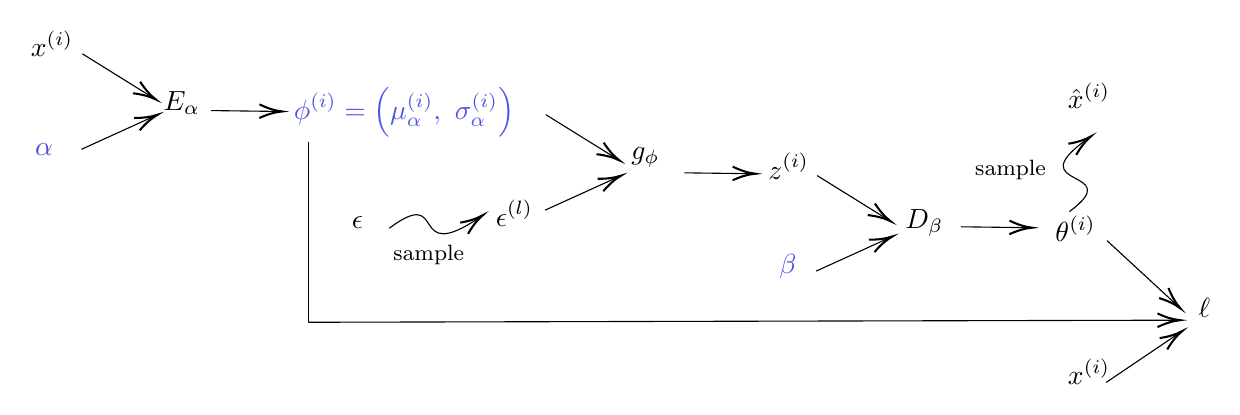
\begin{tikzpicture}[x=0.75pt,y=0.75pt,yscale=-1,xscale=1]
      %uncomment if require: \path (0,230); %set diagram left start at 0, and has height of 230

      %Straight Lines [id:da549284335951172] 
      \draw    (40.09,43.33) -- (73.79,64.28) ;
      \draw [shift={(75.49,65.33)}, rotate = 211.86] [color={rgb, 255:red, 0; green, 0; blue, 0 }  ][line width=0.75]    (10.93,-3.29) .. controls (6.95,-1.4) and (3.31,-0.3) .. (0,0) .. controls (3.31,0.3) and (6.95,1.4) .. (10.93,3.29)   ;
      %Straight Lines [id:da6162521420944999] 
      \draw    (39.67,89.33) -- (74.51,73.49) ;
      \draw [shift={(76.33,72.67)}, rotate = 155.56] [color={rgb, 255:red, 0; green, 0; blue, 0 }  ][line width=0.75]    (10.93,-3.29) .. controls (6.95,-1.4) and (3.31,-0.3) .. (0,0) .. controls (3.31,0.3) and (6.95,1.4) .. (10.93,3.29)   ;
      %Straight Lines [id:da12977974645980606] 
      \draw    (102.09,70.67) -- (134.33,71.09) ;
      \draw [shift={(136.33,71.11)}, rotate = 180.74] [color={rgb, 255:red, 0; green, 0; blue, 0 }  ][line width=0.75]    (10.93,-3.29) .. controls (6.95,-1.4) and (3.31,-0.3) .. (0,0) .. controls (3.31,0.3) and (6.95,1.4) .. (10.93,3.29)   ;
      %Curve Lines [id:da5962854824857341] 
      \draw    (188,127.33) .. controls (216.56,106.1) and (196.3,145.89) .. (231.36,122.24) ;
      \draw [shift={(233,121.11)}, rotate = 145.15] [color={rgb, 255:red, 0; green, 0; blue, 0 }  ][line width=0.75]    (10.93,-3.29) .. controls (6.95,-1.4) and (3.31,-0.3) .. (0,0) .. controls (3.31,0.3) and (6.95,1.4) .. (10.93,3.29)   ;
      %Straight Lines [id:da19986172160423643] 
      \draw    (394.09,102) -- (427.79,122.94) ;
      \draw [shift={(429.49,124)}, rotate = 211.86] [color={rgb, 255:red, 0; green, 0; blue, 0 }  ][line width=0.75]    (10.93,-3.29) .. controls (6.95,-1.4) and (3.31,-0.3) .. (0,0) .. controls (3.31,0.3) and (6.95,1.4) .. (10.93,3.29)   ;
      %Straight Lines [id:da563527517377988] 
      \draw    (393.67,148) -- (428.51,132.16) ;
      \draw [shift={(430.33,131.33)}, rotate = 155.56] [color={rgb, 255:red, 0; green, 0; blue, 0 }  ][line width=0.75]    (10.93,-3.29) .. controls (6.95,-1.4) and (3.31,-0.3) .. (0,0) .. controls (3.31,0.3) and (6.95,1.4) .. (10.93,3.29)   ;
      %Straight Lines [id:da9810030545590435] 
      \draw    (463.42,126.67) -- (495.67,127.09) ;
      \draw [shift={(497.67,127.11)}, rotate = 180.74] [color={rgb, 255:red, 0; green, 0; blue, 0 }  ][line width=0.75]    (10.93,-3.29) .. controls (6.95,-1.4) and (3.31,-0.3) .. (0,0) .. controls (3.31,0.3) and (6.95,1.4) .. (10.93,3.29)   ;
      %Curve Lines [id:da27917860120610793] 
      \draw    (515.67,119.33) .. controls (544.23,98.1) and (490.33,108.78) .. (524.38,84.26) ;
      \draw [shift={(526,83.11)}, rotate = 145.15] [color={rgb, 255:red, 0; green, 0; blue, 0 }  ][line width=0.75]    (10.93,-3.29) .. controls (6.95,-1.4) and (3.31,-0.3) .. (0,0) .. controls (3.31,0.3) and (6.95,1.4) .. (10.93,3.29)   ;
      %Straight Lines [id:da46048578655946304] 
      \draw    (533.75,133.33) -- (567.69,164.66) ;
      \draw [shift={(569.16,166.01)}, rotate = 222.71] [color={rgb, 255:red, 0; green, 0; blue, 0 }  ][line width=0.75]    (10.93,-3.29) .. controls (6.95,-1.4) and (3.31,-0.3) .. (0,0) .. controls (3.31,0.3) and (6.95,1.4) .. (10.93,3.29)   ;
      %Straight Lines [id:da4526948376904725] 
      \draw    (533.33,201.67) -- (568.34,178.03) ;
      \draw [shift={(570,176.91)}, rotate = 145.97] [color={rgb, 255:red, 0; green, 0; blue, 0 }  ][line width=0.75]    (10.93,-3.29) .. controls (6.95,-1.4) and (3.31,-0.3) .. (0,0) .. controls (3.31,0.3) and (6.95,1.4) .. (10.93,3.29)   ;
      %Straight Lines [id:da8633959975997318] 
      \draw    (263.42,72.67) -- (297.13,93.61) ;
      \draw [shift={(298.82,94.67)}, rotate = 211.86] [color={rgb, 255:red, 0; green, 0; blue, 0 }  ][line width=0.75]    (10.93,-3.29) .. controls (6.95,-1.4) and (3.31,-0.3) .. (0,0) .. controls (3.31,0.3) and (6.95,1.4) .. (10.93,3.29)   ;
      %Straight Lines [id:da9054037281263334] 
      \draw    (263,118.67) -- (297.85,102.83) ;
      \draw [shift={(299.67,102)}, rotate = 155.56] [color={rgb, 255:red, 0; green, 0; blue, 0 }  ][line width=0.75]    (10.93,-3.29) .. controls (6.95,-1.4) and (3.31,-0.3) .. (0,0) .. controls (3.31,0.3) and (6.95,1.4) .. (10.93,3.29)   ;
      %Straight Lines [id:da29559166512265533] 
      \draw    (330.09,100.67) -- (362.33,101.09) ;
      \draw [shift={(364.33,101.11)}, rotate = 180.74] [color={rgb, 255:red, 0; green, 0; blue, 0 }  ][line width=0.75]    (10.93,-3.29) .. controls (6.95,-1.4) and (3.31,-0.3) .. (0,0) .. controls (3.31,0.3) and (6.95,1.4) .. (10.93,3.29)   ;
      %Straight Lines [id:da24075226630898383] 
      \draw    (149,85.67) -- (149,172.67) ;
      %Straight Lines [id:da4542808940553933] 
      \draw    (149,172.67) -- (567,171.67) ;
      \draw [shift={(569,171.67)}, rotate = 179.86] [color={rgb, 255:red, 0; green, 0; blue, 0 }  ][line width=0.75]    (10.93,-3.29) .. controls (6.95,-1.4) and (3.31,-0.3) .. (0,0) .. controls (3.31,0.3) and (6.95,1.4) .. (10.93,3.29)   ;

      % Text Node
      \draw (14,31) node [anchor=north west][inner sep=0.75pt]   [align=left] {$\displaystyle x^{( i)}$};
      % Text Node
      \draw (16,85.33) node [anchor=north west][inner sep=0.75pt]  [color={rgb, 255:red, 77; green, 74; blue, 226 }  ,opacity=1 ] [align=left] {$\displaystyle \alpha $};
      % Text Node
      \draw (78,60.33) node [anchor=north west][inner sep=0.75pt]   [align=left] {$\displaystyle E_{\alpha }$};
      % Text Node
      \draw (140.67,58.33) node [anchor=north west][inner sep=0.75pt]  [color={rgb, 255:red, 74; green, 87; blue, 226 }  ,opacity=1 ] [align=left] {$\displaystyle \phi ^{( i)} =\left( \mu _{\alpha }^{( i)} ,\ \sigma _{\alpha }^{( i)}\right)$};
      % Text Node
      \draw (188.67,134) node [anchor=north west][inner sep=0.75pt]  [font=\footnotesize] [align=left] {$\displaystyle \text{\text{sample}}$};
      % Text Node
      \draw (369.33,90) node [anchor=north west][inner sep=0.75pt]   [align=left] {$\displaystyle z^{( i)}$};
      % Text Node
      \draw (374.67,138.67) node [anchor=north west][inner sep=0.75pt]  [color={rgb, 255:red, 77; green, 74; blue, 226 }  ,opacity=1 ] [align=left] {$\displaystyle \beta $};
      % Text Node
      \draw (435.33,117) node [anchor=north west][inner sep=0.75pt]   [align=left] {$\displaystyle D_{\beta }$};
      % Text Node
      \draw (507.67,120) node [anchor=north west][inner sep=0.75pt]   [align=left] {$\displaystyle \theta ^{( i)}$};
      % Text Node
      \draw (469,93.33) node [anchor=north west][inner sep=0.75pt]  [font=\footnotesize] [align=left] {$\displaystyle \text{\text{sample}}$};
      % Text Node
      \draw (513.67,56) node [anchor=north west][inner sep=0.75pt]   [align=left] {$\displaystyle \hat{x}^{( i)}$};
      % Text Node
      \draw (513.67,189) node [anchor=north west][inner sep=0.75pt]   [align=left] {$\displaystyle x^{( i)}$};
      % Text Node
      \draw (576.67,160) node [anchor=north west][inner sep=0.75pt]   [align=left] {$\displaystyle \ell $};
      % Text Node
      \draw (238,112.67) node [anchor=north west][inner sep=0.75pt]   [align=left] {$\displaystyle \epsilon ^{( l)}$};
      % Text Node
      \draw (168.67,120.33) node [anchor=north west][inner sep=0.75pt]   [align=left] {$\displaystyle \epsilon $};
      % Text Node
      \draw (303.33,87.33) node [anchor=north west][inner sep=0.75pt]   [align=left] {$\displaystyle g_{\phi }$};
    \end{tikzpicture}
    \caption{Note that the $\epsilon$ variable was added into the graph, and the blue variables are the parameters we want to backpropagate and optimize. Therefore the path from $\ell$ to $\alpha$ does not directly go through a stochastic node. Note that autograd calculates gradients for $\phi$ while on its way to $\alpha$. But since $\ell$ is directly dependent on $\phi^{(i)}$, we want to make sure to update the $\phi^{(i)}$ directly with a step in the right direction. The rest of the parameters, while they do have their gradients computed, do not need to be updated with a step. A similar figure on a smaller scale can be found in Kigma's workshop presentation in NIPS. } 
    \label{fig:reparam_trick}
  \end{figure}

  Another advantage is that this is more general. Although we must meet the conditions that the posterior $p_\phi (z \mid x)$ should be an absolutely continuous distribution that can be modeled as the transformation of a simple random variable $\epsilon$, since any distribution that is differentiable with respect to its parameters can be reparamaterized by inverting the multivariate CDF function and applying the implicit method. 

  In order to see how the gradients are calculated, recall the following theorem. 

  \begin{theorem}[Change of Basis]
    We have 
    \begin{equation}
      \log q_\phi (z \mid x) = \log p(\epsilon) - \log \bigg| \mathrm{det} \bigg( \frac{\partial z}{\partial \epsilon}\bigg)\bigg| 
    \end{equation}
    where $\partial z / \partial \epsilon$ denotes the Jacobian matrix computed through $g_\phi(x, \epsilon)$. 
  \end{theorem}
  
  \begin{corollary}
    This applied to the affine function $g_\phi$ above defined for the log-variance gives 
    \begin{equation}
      \frac{\partial z}{\partial \epsilon} = \mathrm{diag}(\sigma) \implies \log \bigg| \mathrm{det} \bigg( \frac{\partial z}{\partial \epsilon}\bigg)\bigg| = \sum_i \log \sigma_i
    \end{equation}
  \end{corollary}

  \begin{corollary}[Auto-Encoding VB (AEVB) Algorithm]
    Applying the reparamaterization trick to the gradient of the ELBO gives the following corollary. 
    \begin{equation}
      \nabla_\phi \elbo(x, \phi, \theta) = \mathbb{E}_{p(\epsilon)}[\nabla_\phi \log p_\theta (x \mid z) - \nabla_\phi \log q_\phi (z \mid x) + \nabla_\phi \log p(z)]
    \end{equation}
    Therefore we can unbiasedly approximate the gradient by sampling $L$ points $\epsilon^{(1)}, \ldots, \epsilon^{(L)}$ from $p(\epsilon)$, transforming them to $z^{(1)}, \ldots, z^{(L)}$ through the function $g_\phi$, and finally computing the gradient of the log posterior (which is easy since we know the closed form of the conditional distribution given $z$), and finally averaging them. 
    \begin{align*}
      \nabla_\phi \elbo(x, \phi, \theta) & \approx \frac{1}{L} \sum_{l=1}^L [\nabla_\phi \log p_\theta (x \mid z^{(l)}) - \nabla_\phi \log q_\phi (z^{(l)} \mid x) + \nabla_\phi \log p(z^{(l)})] \\
                                         & = \frac{1}{L} \sum_{l=1}^L [\nabla_\phi \log p_\theta (x \mid g_\phi (\epsilon^{(l)}, x)) - \nabla_\phi \log q_\phi (g_\phi (\epsilon^{(l)}, x) \mid x) + \nabla_\phi \log p(g_\phi (\epsilon^{(l)}, x))]
    \end{align*}
    which is guaranteed to converge by the law of large numbers, and furthermore we can do this for any batch size $L$. 
  \end{corollary}


  Really the VAEs were just a straightforward application of CAVI with the reparamaterization trick, plus the extra variables $\alpha, \beta$ that are used to generate the $\theta, \phi$. 

  \begin{algo}[Implementation of VAE]
    To see an implementation of a VAE with PyTorch, see \href{code/vae.html}{here}. 
  \end{algo} 

\subsection{Importance Weighted Autoencoders}

\subsection{Fisher Autoencoders}

\subsection{Conditional VAEs}

  Note that once our VAE is trained, we have no control on the data generation process. That is, if we want to generate only the digit 2, we can't since we must just sample from the Gaussian $p(z)$ in the latent space. Therefore, conditioning all the distributions on what we want is the objective of \textit{conditional VAEs}, which uses the \textit{conditional ELBO}. 

  \begin{definition}[Conditional ELBO]
    The \textbf{conditional ELBO} of $x, \theta, \phi$ given some conditioning vector $c$\footnote{Analogous to the digit we want in MNIST.}, is defined 
    \begin{equation}
      \mathbb{E}_{q_\phi(z \mid x)} \big[ \log p_\theta(x \mid z,c) - \mathrm{KL}(q_\phi (z \mid x,c) || p(z \mid c)) \big] 
    \end{equation}
  \end{definition}

\bibliographystyle{alpha}
\bibliography{./bibfile}
\end{document}

